\section{Regressione}
\label{sec:regressione}

Parlando di \textbf{regressione}, si ha un problema impostato allo stesso modo
di quelli di classificazione binaria o multiclasse, ma l'\textit{output} è un
\textbf{nuemro reale}.

\textbf{Nota:} quando all'interno della nostra rete abbiamo dei valori categorici, sappiamo che per
gestirli utilizziamo la tecnica del \textbf{one hot encoding}. Ma quando abbiamo valori numerici, come gestiamo questi dati?
Potremmo avere dati che hanno \textit{scale diverse, unità di misura diverse}, ecc\dots. Questi rendono abbastanza
complicato il lavoro della rete. Per questo motivo, è necessario \textbf{normalizzare} i dati.

\subsection{Boston Housing Price}
\label{subsec:boston_housing_price}

Il dataset \textbf{Boston Housing Price} è un dataset che contiene 506 esempi
di case nella zona di Boston. Ogni esempio è composto da 13 \textit{feature}
che descrivono la casa e il prezzo della casa. Questo dataset è stato
utilizzato per la prima volta nel 1978, ma è ancora utilizzato per testare i
modelli di regressione, ed è proprio quello che faremo noi.

\begin{lstlisting}[language=Python, caption=Caricamento del dataset]
    from keras.datasets import boston_housing
    (train_data, train_targets), (test_data, test_targets) = boston_housing.load_data()
\end{lstlisting}

\subsubsection{Normalizzare i dati}
\label{subsubsec:normalizzare_dati}

La normalizzazione consiste nel portare i valori numerici di un dataset tutti
sulla stessa scala. Abbiamo due modi per fare questo processo di
normalizzazione:
\begin{itemize}
    \item MinMax Normalization: La MinMax Normalization è una tecnica di normalizzazione
          dei dati che consiste nel portare tutti i valori di un dataset su una scala
          compresa tra 0 e 1. Questa tecnica è utile quando i dati hanno scale diverse e
          si vuole portarli tutti sulla stessa scala per facilitare l'elaborazione da
          parte della rete neurale. Per applicare la MinMax Normalization, si utilizza la
          seguente formula per ogni valore del dataset: Viene usata ma \textbf{non è
              proprio approrpiata.}
          \begin{equation}
              x_{norm} = \frac{(x - x_{min})}{(x_{max} - x_{min})}
          \end{equation}
    \item Normalizzazione Statistica: Si utilizzano la \textbf{media} e la
          \textbf{deviazione standard}. Questa tecnica è utile quando i dati hanno scale
          diverse e si vuole portarli tutti sulla stessa scala per facilitare
          l'elaborazione da parte della rete neurale.
          \begin{lstlisting}
        mean = train_data.mean(axis=0)
        train_data -= mean
        std = train_data.std(axis=0)
        train_data /= std

        test_data -= mean
        test_data /= std
    \end{lstlisting}
          Questo porta un \textbf{centramento} intorno allo 0. \textbf{Nota importante:}
          Da notare le righe \textit{6 e 7} che applicano la normalizzazione dei dati
          \textbf{anche sul test set}. Questa cosa si fa? La risposta è \textbf{NON
              ABBIAMO MAI I TEST DATA.}

          Praticamente stiamo facendo l'assunzione che i dati vengano dalla
          \textbf{stessa distribuzione}. Poiché i risultati del test set probabilmente
          saranno su una scala diversa rispetto a quelli che abbiamo dal training set e i
          risultati che otteniamo dal nostro modello potrebbero essere su una scala diversa
          rispetto a quella del training. Quindi, questo va fatto solo se si ha la certezza
            che i dati provengano dalla stessa distribuzione.
\end{itemize}

\subsubsection{Costruzione della rete}
\begin{lstlisting}[language=Python]
def build_model():
    # Because we will need to instantiate
    # the same model multiple times,
    # we use a function to construct it.
    model = models.Sequential()
    model.add(layers.Dense(64, activation='relu',
                input_shape=(train_data.shape[1],)))
    model.add(layers.Dense(64, activation='relu'))
    model.add(layers.Dense(1))
    model.compile(optimizer='rmsprop', loss='mse', metrics=['mae'])
    return model
\end{lstlisting}

Piccole note su questo codice:
\begin{enumerate}
    \item L'ultimo livello ha un solo nodo di output
    \item Non ha una funzione di attivazione
    \item Sta usando la metrica \textbf{MAE}: Mean Absolute Error e la loss \textbf{MSE}: Mean Squared Error
\end{enumerate}

\subsubsection{Validation con pochi data point}
\label{subsubsec:validation_pochi_data_point}

\textbf{Spiegazione al volo della K-Fold validation}: La K-Fold validation è una tecnica di
validazione che consiste nel dividere il dataset in \textbf{K parti} e utilizzare una di 
queste parti come \textbf{validation set} e le altre come \textbf{training set}. 

\subsubsection{Visualizzare i risultati}

\begin{lstlisting}[language=Python]
average_mae_history = [
    np.mean([x[i] for x in all_mae_histories]) for i in range(num_epochs)]

import matplotlib.pyplot as plt

plt.plot(range(1, len(average_mae_history) + 1), average_mae_history)
plt.xlabel('Epochs')
plt.ylabel('Validation MAE')
plt.show()

\end{lstlisting}

\textbf{Nota:} Solitamente i primi punti in una task di regressione \textbf{sono fuori scala}. Conviene scartarli e non 
contarli nella big picture finale.

\begin{figure}[H]
    \centering
    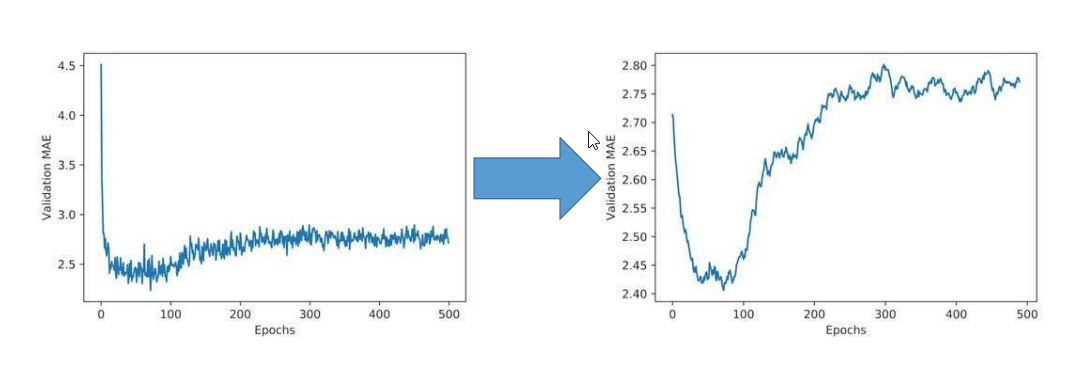
\includegraphics[scale=0.5]{images/mae.png}
    \caption{Grafico MAE}
    \label{fig:mae}
\end{figure}

\subsection{Overfitting}
\label{subsec:overfitting}

Formalizziamo al volo il problema:

\begin{equation}
    \min_{w} [loss(y,NN(x|w))]
\end{equation}

Cioe vogliamo minimizzare in funzione dei pesi la funzione che ha come parametri la \textbf{vera y} e 
la \textbf{y predictata} usando il nostro input \textbf{x} e i pesi \textbf{w}.

La tecnica che vediamo è la \textbf{regolarizzazione}.

\subsubsection{Regolarizzazione}

La regolarizzazione è una tecnica che non fa altro che \textbf{modificare la funzione che vogliamo approssimare}.
Questo rende i pesi della rete più piccoli, il che rende la distribuzione dei valori \textit{più regolare.}
\begin{equation}
    \min_{w} [loss(y,NN(x|w)) + R(w)]
\end{equation}

Abbiamo due tipi di regolarizzazione:
\begin{itemize}
    \item L1 Regularization: \textit{vecchia loss function} + $\lambda \sum_i|w_i|$, cioè aggiunge la somma dei valori assoluti dei pesi.
    \item L2 Regularization: \textit{vecchia loss function} + $\lambda \sum_i w_i^2$, cioè aggiunge la somma dei valori dei pesi al quadrato.
\end{itemize}

Queste due tecniche rendono \textit{il modello più sensibile la noise e alla varianza dei dati.}
\begin{itemize}
    \item L2: Rende i pesi più piccoli
    \item L1: Rende i pesi più sparsi (più 0, in pratica)
\end{itemize}

\begin{lstlisting}[language=Python]
from keras import regularizers
l2_model = models.Sequential()
l2_model.add(layers.Dense(8, kernel_regularizer=regularizers.l2(0.001),
    activation='relu'
    , input_shape=(10000,)))
l2_model.add(layers.Dense(8, kernel_regularizer=regularizers.l2(0.001),
            activation='relu'))
l2_model.add(layers.Dense(1, activation='sigmoid'))
\end{lstlisting}


\textbf{Nota:} si può fare una combinazione tra L1 e L2.

\begin{lstlisting}[language=Python]
from keras import regularizers
# L1 regularization
regularizers.l1(0.001)
# L1 and L2 regularization at the same time
regularizers.l1_l2(l1=0.001, l2=0.001)
\end{lstlisting}

\begin{figure}[H]
    \centering
    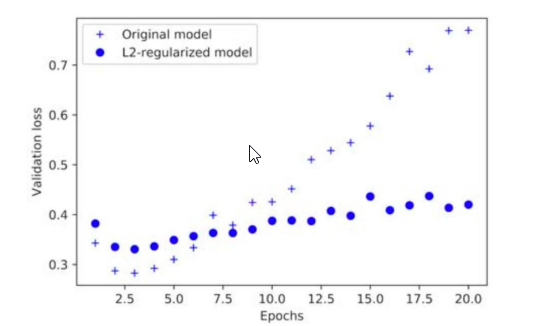
\includegraphics[scale=0.5]{images/l2reg.png}
    \caption{Grafico Regularization L2}
    \label{fig:regularization}
\end{figure}

Quindi, alla fine, \textbf{early stopping} e \textbf{diminuire grandezza rete} non vengono fatti con 
leggerezza e non sono spesso soluzioni applicabili.

\subsection{Dropout}
\label{subsec:dropout}

In teoria, questa tecnica prevede il rimuovere \textbf{durante il training} alcuni nodi della rete in modo casuale seguendo 
una specifica distribuzione (si setta il valore di 0). L'effetto è quello di rendere 
la rete più confusa, e quindi più robusta. \textbf{Quando si fa il testing} si va ad utilizzare l'intera rete senza
troncamenti di connessioni.

\textbf{Per quale motivo funziona?} La rispota è \textbf{BOH}. Il fatto è che \textbf{funziona} ed è uno standard. Quindi praticamente 
in ogni NN si utilizza la tecnica del \textit{dropout}.

\begin{lstlisting}[language=Python]
dpt_model = models.Sequential()
dpt_model.add(layers.Dense(16, activation='relu', input_shape=(10000,)))
#Probabilita di rendere 0 un nodo del layer con probabilita 0.5
dpt_model.add(layers.Dropout(0.5))
dpt_model.add(layers.Dense(16, activation='relu'))
dpt_model.add(layers.Dropout(0.5))
dpt_model.add(layers.Dense(1, activation='sigmoid'))
dpt_model.compile(optimizer='rmsprop',
    loss='binary_crossentropy',
    metrics=['acc'])
\end{lstlisting}

\begin{figure}[H]
    \centering
    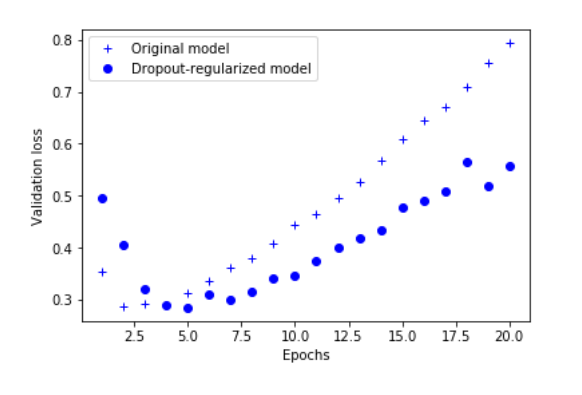
\includegraphics[scale=0.5]{images/dropout.png}
    \caption{Grafico Dropout}
    \label{fig:dropout}
\end{figure}

\newpage